\documentclass[a4paper,12pt]{article}
\usepackage[catalan]{babel}
\usepackage[utf8]{inputenc}
\usepackage{amsfonts}
\usepackage[colorlinks=true]{hyperref}
\usepackage[left=2.5cm,right=2.5cm]{geometry}
\usepackage{graphicx}
\usepackage[labelformat=empty]{caption}

\title{L'Esfera Terrestre \\ Activitats \\ {\small \today  } }
\author{Daniel Ramos \footnote{E-mail: \texttt{daniel.ramos@mmaca.cat}}\\MMACA (Museu de Matemàtiques de Catalunya)}

\date{}

\pagestyle{empty}

\begin{document}
\maketitle \thispagestyle{empty}

Aquestes activitats han estat dissenyades per a ser realitzades amb els materials, pòsters i software del expositor ``L'Esfera Terrestre''. Aquest material es dóna com a referència bàsica, es pot elaborar en forma de conferència, o es pot imprimir i penjar sobre les parets al costat dels pòsters i expositors. Aquest material no ha estat revisat exhaustivament. Pot contenir errors i faltes. Llegiu-ho amb cura abans de fer-ho servir en públic i contacteu l'autor per qualsevol qüestió o error.

\vspace{4em}
L'ús proposat és el següent: Utilitzeu la secció 1 com a material introductori, prop d'una taula amb el glòbus i les eines. Mostreu cada secció 2-7 en un plafó al costat de cada pòster corresponent en una paret propera. Mostreu la secció 8 al costat de l'ordinador, a fi de fer-ho servir després de veure els pòsters. Utilitzeu la secció 9 com a material complementari per al públic interessat.


%\thanks{Universitat Autònoma de Barcelona, Departament de Matemàtiques - 80193 Bellaterra, Barcelona (Spain)- \\ E-mail:
%\texttt{dramos@mat.uab.cat} . }


\newpage
\section{Què és un mapa?}
Un \emph{mapa} o \emph{projecció cartogràfica} és una representació plana de la superfície de la Terra. Hi ha infinites maneres de representar la Terra sobre un pla, però totes elles distorsionaràn la seva aparença d'una o una altra manera. Depenent del propòsit del mapa, ens pot interessar preservar fidelment algunes propietats tot i assumint que en perdrem unes altres. Per exemple, en un mapa per a la navegació és molt important mantenir fidelment l'angle de la nostra ruta amb el Nord, ja que el podrem comparar amb la direcció del Nord en la nostra brúixola per a orientar-nos. Si necessitem, per exemple, representar regions climàtiques de la Terra, ens sera molt més adient un mapa que no distorsioni les àrees.


\begin{itemize}
 \item Mireu el glòbus terraqüi sobre la taula, i els mapes que hi ha exposats a les parets. Tots els mapes tenen la forma de la Terra? Podeu notar o descriure la distorsió de cada mapa? 
 \item Mireu la graella que hi ha dibuixada sobre el glòbus i sobre els mapes. Per a què serveix? Ens ajuda a veure la distorsió?
 
\end{itemize}

\subsection*{Coordenades}
El sistema de coordenades de la Terra és una manera de localitzar un punt mitjançant dos nombres: una \emph{longitud} ($\lambda$) i una \emph{latitud} ($\phi$). A la Terra, les referències fixes són els pols Nord i Sud (l'eix de la Terra), el pla equatorial (perpendicular a l'eix), i el semiplà que conté el Royal Observatory de Greenwich i l'eix de la Terra. Donat un punt de la Terra $p$, la seva longitud és l'angle entre el semiplà que conté $p$ i l'eix de la Terra i el semiplà de Greenwich. La latitud és l'angle entre la línia que uneix el centre de la Terra amb $p$ i el pla equatorial.

\begin{itemize}
 \item Identifiqueu longitud i latitud en el model transparent de la taula.
\end{itemize}
Línies d'igual longitud s'anomenen \emph{meridians}, i línies d'igual latitud s'anomenen \emph{paral·lels}. Algunes d'aquestes línies es poden dibuixar per a formar una graella anomenada \emph{gratícula}. El glòbus i els mapes tenen una gratícula espaiada 10º en cada coordenada.

Sobre el glòbus, la distància entre punts es pot mesurar com una longitud (en kilòmetres) o com l'angle de l'arc definit per aquests dos punts i el centre de la Terra com a vèrtex (en graus o radians). Recodeu que 
$ arc = angle \cdot radi $
(expressant l'angle en radians, no en graus, i l'arc i el radi en unitats de longitud (km)).

\begin{itemize}
 \item Intenteu trobar de manera aproximada les coordenades d'algunes ciutats sobre el glòbus i sobre els mapes.
 \item Utilitzeu el regle flexible per a mesurar algunes distàncies. Observeu que hi ha dues escales: en quilòmetres i en graus.
\end{itemize}





\newpage
\section{La projecció Plate-Carrée}
Aquesta és potser la projecció més fàcil. Només cal escriure la longitud i la latitud com les coordenades $x$ i $y$ del pla. Per tant, la gratícula queda formant una graella quadrada uniforme. És aquesta representació fidel a la realitat?

\begin{itemize}
 \item Cada quadrat de la gratícula representa 10ª sobre la Terra. Però, és la gratícula sobre la Terra ``quadrada''? Comproveu la forma d'un ``quadrat'' de la gratícula prop de l'equador i prop del pol Nord al glòbus. Tenen costats d'igual distància? Quant mesura un arc de paral·lel de 10º a l'equador? Quant mesura a latitud 70ºN? 
 \item Funciona el regle flexible sobre aquest mapa?
\end{itemize}
Per a ser més fidel a la realitat, la gratícula no hauria de ser una graella quadrada.




 
\newpage
\section{La projecció de Mercator}
Aquesta projecció va ser inventada per Gerardus Mercator en 1569, i és sense cap mena de dubte la projecció cartoogràfica més important de la Història. La majoria de mapes de propòsit general utitlitzen aquesta projecció. Observeu amb cura un ``quadrat'' de la gratícula sobre el glòbus terraqüi, prop dels pols. Aquests ``quadrats'' semblen més com rectangles. La projecció de Mercator és una deformació vertical de la projecció Plate-Carrée. Ja que els paral·lels apareixien més llargs del que són en realitat, els meridians han estat estirats la mateixa quantitat, de manera que ara el mapa esta alargat en vertical i en horitzontal la mateixa quantitat en cada punt. Les regions i les àrees són molt distorsionades, però d'altra banda hem aconseguit una característica molt important: les formes i els angles s'han preservat.

Una característica clau per a la navegació és la següent: Imagineu que voleu navegar des s'una ciutat fins a una altra a través de l'oceà. Podeu traçar la línia recta que uneix aquestes ciutats en el mapa de Mercator. Aquesta línia (anomenada \emph{loxodroma} o línia de rumb) forma un angle constant amb els meridians verticals, que apunten al Nord. Donat que els angles es preserven, aquest és el veritable angle que heu de mantenir constant amb la brúixola del vostre vaixell (encara que hauríeu de corregir la petita diferència entre Nord magnètic i geogràfic). Així, el mapa de Mercator permet, i ha permès durant segles, trobar un camí entre dos punts de la Terra. Compte: aquesta loxodroma és només un camí fàcil de seguir, no el més curt!


\begin{itemize}
 \item Imagineu que sou al segle XVI i que voleu navegar des de Càdis (Sud d'Espanya) fins a Caracas (avui Venezuela) en la vostra caravel·la. Quina és la ruta més fàcil de seguir (loxodroma)? Useu el transportador pla.

 \item Imagineu que voleu volar avui dia des de Atenes (Grècia) fins a Los Angeles (USA). Quina loxodroma uneix aquestes dues ciutats?
 
 Si realment preneu un avió fent ruta directa des de Atenes fins Los Angeles, veureu que voleu sobre una gran extensió nevada. És Groenlàndia. Per què? Busqueu la ruta més curta al glòbus.

 \item Utilitzeu els transportadors esfèric i pla per a comprovar la igualtat d'angles sobre loxodromes en el mapa i en el glòbus.
\end{itemize}



\newpage
\section{La projecció de Gall-Peters}
La projecció de Mercator intenta arreglar la distrorsió de la projecció Plate-Carrée corregint els angles, però això distorsona àmpliament les àrees. Altres projeccions, com la de Gall-Peters, són dissenyades per a preservar les àrees. La projecció de Gall-Peters és coneguda com la projecció ``del tercer món'', perquè països de l'Àfrica i de Sudamèrica (i totes les regions prop de l'equador) tenen un lloc preeminent. Si l'Àfrica sembla més gran que l'Europa, és perquè \emph{realment és} més gran (les àrees són correctes). Tanmateix, la forma no es preserva. L'Àfrica no és tan prima i allargassada com sembla en aquest mapa.

\begin{itemize}
 \item Quin continent és més gran, Nordamèrica o Àfrica? Contesteu mirant la projecció de Gall-Peters. Diríeu el mateix mirant la projecció de Mercator? (Resposta: Nordamèrica fa uns $24.709.000\ \mathrm{km}^2$ i Africa uns $30.221.532\ \mathrm{km}^2$.)

 \item Utilitzeu les siluetes d'escuma per a comparar els tamanys dels continents en el mapa amb els verdaders continents esfèrics. Encaixen? Què passa amb l'Antàrtida?
\end{itemize}



\newpage
\section{La projecció Azimutal Equidistant}
Aquest és el ``mapa d'aeroport''. Al centre del mapa és Barcelona (però podríem posar qualsevol punt de la Terra). Una vegada fixat el centre, dibuixem punts a distàncies iguals de Barcelona sobre circumferències concèntriques al voltant del centre, utilitzant la distància com a radi. Així, la distància des de Barcelona fins a qualsevol punt del món es mostra correctament en aquest mapa (però només distàncies des de Barcelona!). L'angle entre el radi que uneix Barcelona amb el punt de destí i el Nord del mapa (direcció vertical) també és correcte. Així, aquest és un mapa molt convenient de tenir a l'aeroport de Barcelona, perquè dona una bona idea de com de llarg serà el viatge i sobre quins països volarem. També podem veure com de lluny són diferents ciutats.

Podeu utilitzar el regle flexible sobre aquest mapa, però només si mesureu distàncies des de Barcelona; en cas contrari la mesura serà errònia.

\begin{itemize}
 \item Com de lluny són Nova York (USA), Ciutat del Cap (Sudàfrica) i Tòquio (Japó) de Barcelona? Quina de les tres és més lluny?
 \item Quin és el diàmetre d'aquest mapa?
 \item Quants països podem visitar viatjant menys de 10.000 km? 
 \item Les antípodes de Barcelona (el punt de la Terra diametralment oposat a Barcelona) és un punt de l'oceà Pacífic, a prop de Nova Zelanda. On és aquest punt al mapa? On és Nova Zelanda?
\end{itemize}



\newpage
\section{La projecció Gnomònica}
Aquest mapa sembla enormement distorsionat. Tanmateix, té una propietat única: tots els camins més curts sobre la Terra (geodèsiques) hi són representats com a línies rectes. Així, si volem que el camí més curt entre dos punts sigui (sembli) una línia recta, hem de distorsionar tant el mapa. A més, no es pot mostrar tota la Terra, només una petita porció menor que un hemisferi. El centre de la projecció s'ha pres a Barcelona. Podeu aconseguir aquest mapa projectant cada punt de la superfície de la Terra des del centre de la Terra sobre un pla tangent a Barcelona.

\begin{itemize}
 \item Trobeu el camí més curt des de Jerusalem (Israel) fins a La Habana (Cuba). Passa per sobre de l'Àfrica? Diríeu el mateix mirant les altres projeccions?
 \item Quina forma adopten paral·lels i meridians?
\end{itemize}





\newpage
\section{La projecció de Mollweide}
Aquesta projecció omple una el·lipse d'eixos en proporció 2:1. Això resol parcialment un problema comú a totes les projeccions cilíndriques (com ara Plate-Carrée, Mercator, Gall-Peters i altres), el fet de que els pols no són representats a un únic punt. El pol Nord en la projecció de Plate Carrée correspon a tota la vora superior del mapa rectangular. Això distorsiona enormement les regions al voltant dels pols, com l'Antàrtida. La projecció de Mollweide resol això i en redueix la distorsió. Més encara, la projecció de Mollweide preserva àrees, de manera que la distorsió és només en forma, no en tamany. Finalment, la seva forma arrodonida recorda la esfericitat de la Terra, cosa que no és tan aparent en altres mapes rectangulars.


\begin{itemize}
 \item Com es representen els paral·lels i els meridians?
 
 
  \item Compareu aquesta projecció amb la de Gall-Peters. Ambdues preserven àrees. Quina creieu que distorsiona menys la forma real de la Terra? Utilitzeu els perfils de escuma i el globus per a comparar els continents.
  
\end{itemize}



\newpage
\section{Com podem mesurar la distorsió?}
La distorsió d'un mapa és una magnitud complicada que no pot ser mesurada per un únic nombre. Tanmateix, el matemàtic francès Nicolas Auguste Tissot va idear en 1859 un mètode gràfic per a mostrar la distorsió produïda a qualsevol punt d'un mapa. Imagineu un petit cercle al voltant d'un punt de la Terra. Si projectem aquest cercle sobre el mapa, no el veurem com a un cercle, degut a la distorsió. Si el cercle és prou petit (un cercle infinitesimal), el que veurem serà una el·lipse (una el·lipse infinitesimal). Podem mostrar aquesta el·lipse magnificada per a veure-la sobre el mapa. Aquesta el·lipse s'anomena \emph{indicatriu de Tissot} del mapa, i dóna diversa informació sobre la distorsió.

\begin{figure}[h]
 \begin{center}
  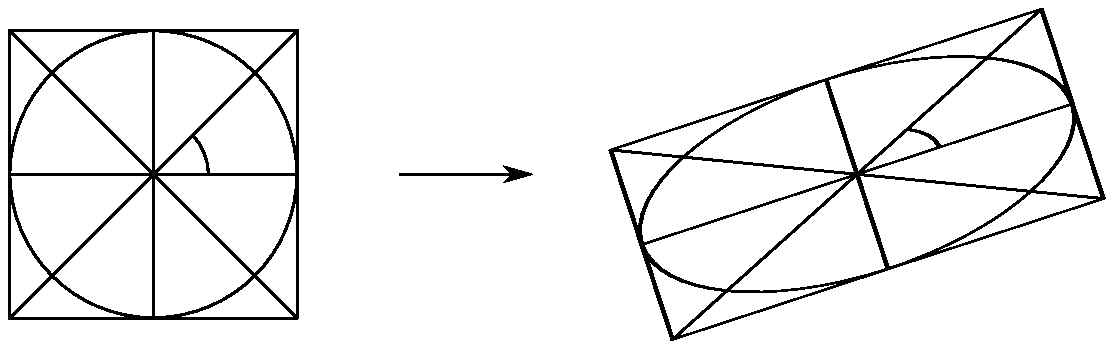
\includegraphics[width=0.7\textwidth]{tiss_diagram} 
\caption{Un cercle infinitesimal es projecta en una el·lipse infinitesimal.}%\label{tiss_diagram}
 \end{center}
\end{figure}
\vspace{-1em}
\begin{itemize}
 \item Mireu la pantalla amb el programa. Podeu sel·leccionar el mapa a les pestanyes superiors. Quan moveu el cursor sobre el mapa, la el·lipse de Tissot apareix sobre el mapa. Si feu clic deixareu una el·lipse impresa. Podeu triar el tamany de les el·lipses o esborrar-les totes.
 
\end{itemize}



\paragraph{Direccions principals.} 
Podem pensar en la distorsió com a contreure i expandir la Terra sobre un mapa. Tanmateix, podem contreure el mapa en una direcció i expandir-lo en una altra, i això de manera diferent en cada punt. Els dos eixos de l'el·lipse de Tissot indiquen les \emph{direccons principals}, són aquelles direccions on la expansió és màxima i mínima. Una el·lipse molt allargada significa que la distorsió és molt diferent d'una direcció a una altra.



\begin{itemize}
 \item Quins mapes tenen el·lipses més extremes? Quina aparença tenen?
 \item Com és la el·lipse al pol Nord en la projecció de Plate-Carrée? On és el pol Nord? 
 \item Són les direccions prncipals sempre les mateixes que les direccions dels paral·lels i meridians?
\end{itemize}



\paragraph{Conformitat.} Una el·lipse de Tissot amb eixos iguals (una circumferència) significa que la distorsió és igual de gran en totes les direccions des d'aquell punt. Així, qualsevol forma (com la línia de la costa) al voltant d'aquest punt s'expandeix uniformement en totes les direccions, i per tant la forma es preserva. Un mapa que conserva la forma en tots els punts se'n diu \emph{conforme}. Observeu en el diagrama anterior que quan l'el·lipse de Tissot és un cercle, tots els angles al voltant d'aquest punt es conserven iguals. \emph{Els mapes conformes preserven els angles}.


\begin{itemize}
 \item Quan l'el·lipse de Tissot és un cercle, la vora de l'el·lipse es torna verda. Trobeu en cada mapa aquells  punts on el mapa és conforme. 
 \item Què és especial en el mapa de Mercator? Quant es distorsionen els angles? i les àrees?
\end{itemize}

\paragraph{Àrea.} 
L'àrea de les el·lipses ens diu si la distorsió mitjana és expansiva o contractant. Si un petit cercle de radi $r$ (d'àrea $\pi r^2$) és projectat en una el·lipse de semieixos $a$ i $b$ (d'àrea $\pi a b$), aleshores la condició $ab=r^2$ significa que l'àrea de l'el·lipse és la mateixa que la del cercle, i per tant el mapa no distorsiona l'àrea en aquest punt (el que es contreu en una direcció es compensa amb el que s'expandeix en una  altra). Un mapa que conserva l'àrea en cada punt es diu \emph{equivalent}.

Si un punt en un mapa preserva tant la forma com l'àrea (és conforme i equivalent), aquest punt es diu que és a \emph{escala real}. Aquest punt es reeresenta sobre el mapa sense cap tipus de distorsió. Un important teorema en geometria diu que no n'hi ha cap mapa amb tots els punts a escala real, és a dir, no existeix el mapa perfecte.

\begin{itemize}
 \item Quan l'àrea es perserva, l'interior de l'el·lipse es torna verd. Quins mapes dels que mostrem són equivalents? Quina és l'àrea de tot el mapa en aquests casos?
 
 \item Compareu les àrees d'Àfrica i de Groenlàndia. Useu primer la projecció de Gall-Peters. Preneu una mida mitja o petita per a les el·lipses. Quantes podeu posar sobre Groenlàndia? i sobre Àfrica? Ara repetiu-ho en la projecció de Mercator. Recordeu: les el·lipses de Tissot poden semblar diferents, però \emph{reprenenten el mateix disc sobre la Terra}.
 
 Com més petit preneu el disc, millor és l'aproximació. El fet és que Àfrica és 14.2 vegades més gran que Groenlàndia. Quin dels dos mapes reflexa millor aquesta proporció?
 

 \item Què és més gran, Groenlàndia o Austràlia? Podeu contestar mirant només a la projecció Plate-Carrée? I fent servir les el·lipses de Tissot?

 \item Tant la projecció de Gall-Peters com la de Mollweide són equivalents. Quina de les dues distorsiona menys la forma?


\end{itemize}



%\begin{figure}[!h]
 \begin{center}
  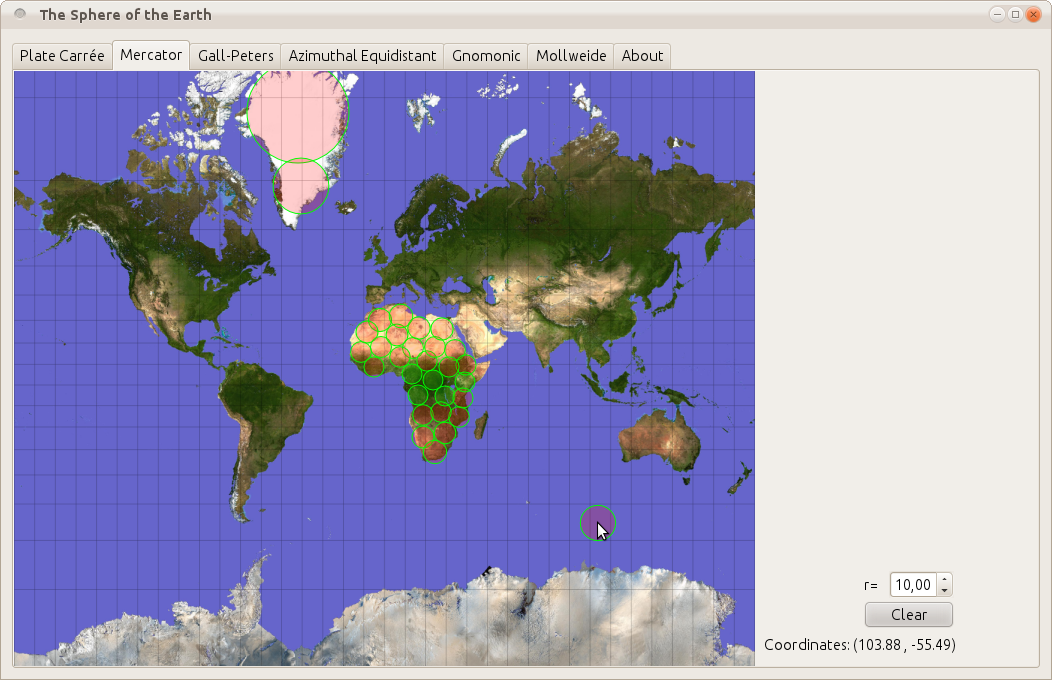
\includegraphics[width=0.7\textwidth]{merc1.png} 
  
{Comparació entre l'àrea d'Àfrica i de Groenlàndia en la projecció de Mercator.}
 \end{center}
%\end{figure}




\newpage
\section{Dins les matemàtiques}
\textsf{Aquesta secció fa servir matemàtiques de nivell superior. Llegiu-ho al vostre risc!} \\

Una projecció és una funció que envia cada parell de coordenades en l'esfera $\mathbb S$ en un parell de coordenades del pla $\mathbb R^2$,
$$\begin{array}{rccc}
   F: &\mathbb S & \longrightarrow & \mathbb R^2 \\
  & (\lambda, \phi) & \mapsto & (x,y)
  \end{array}
$$
on $\lambda$ és la longitud i $\phi$ la latitud. Aquesta funció es pot aproximar per l'aplicació diferencial $dF$
$$\begin{array}{rccc}
   dF_p: & T_p \mathbb S & \longrightarrow & \mathbb R^2 
  \end{array}
$$
que envia el pla tangent a l'esfera en $p$ en el pla $\mathbb R^2$ centrat en $F(p)$. El pla tangent es pot pensar com l'espai de direccions del punt $p$, i el cercle unitari del pla tangent en $p$ representa el conjunt de totes les direccions unitàries des de $p$. L'el·lipse de Tissot és la imatge per $dF$ del cercle unitari en $T_p\mathbb S$. Així, l'el·lipse de Tissot és una representació de \emph{com les direccions des de $p$ són distorsionades}.

\begin{figure}[h]
 \begin{center}
  \def\svgwidth{ 0.85 \textwidth}
\input{df.pdf_tex}
\caption{La funció $F$ i la seva diferencial $dF$.}
 \end{center}
\end{figure}

Hi ha dues direccions perpendiculars a la Terra que també son perpendiculars sobre el mapa. Per veure això, considerem una línia recta $r$ en el pla tangent que passi per $p$, i una semirrecta $t$ amb origen a $p$, perpendicular a $r$. Considerem les seves imatges $r's'$ i $t'$ en el mapa, que es tallen en $p'=F(p)$, no necessàriament de manera perpendicular. Suposem per exemple que $r'p't'$ és un angle agut i que $t'p's'$ és obtús. Ara imaginem que prenem l'angle recte $rpt$ i el rotem al voltant de $p$, començant amb l'angle $rpt$ i terminant en $tps$. A la banda del mapa, hem començat amb l'angle agut $r'p's'$ i hem acabat amb l'angle obtús $t'p's'$, per tant, en algun punt intermig hem tingut un angle recte com a imatge.


\begin{figure}[ht]
 \begin{center}
  \def\svgwidth{ 0.85 \textwidth}
\input{diagonalize.pdf_tex}
\caption{Les direccions principals són perpendiculars.}
 \end{center}
\end{figure}

Aquestes dues direccions són les direccions principals, representades per dos vectors unitaris perpendiculars. La imatge d'aquests dos vectors donen les direccions principals sobre el mapa, i la longitud d'aquestes imatges, $a$, $b$, donen els semieixos de l'el·lipse de Tissot. Si $a=b$ l'el·lipse és un cercle, totes les direccions es dirtorsionen per igual i el mapa és conforme en aquest punt. Si $ab=1$, l'el·lipse té la mateixa àrea que el disc unitari del pla tangent. Utitlitzant un disc infinitesimal obtenim l'àrea infinitesimal de l'esfera, i per tant el mapa és equivalent en aquest punt.

En un llenguatge formal, diem que l'aplicació diferencial és una aplicació lineal que es pot diagonalitzar respecte de la mètrica de l'esfera, els vectors propis donen les direccions principals i els valors propis donen els semieixos de l'el·lipse de Tissot. La condició de conformitat és que $dF$ sigui un múltiple de la matriu identitat, i la condició d'equivalència (preservar àrees) és que $det(dF)=1$. Satisfer ambdues condicions a tot punt implicaria qhe $F$ és una isometria, cosa que és impossible degut al Teorema Egregi de Gauss.

 
 
\end{document}

